\section{OS Concepts}

\paragraph{OS Invocation}
\begin{itemize}
	\item OS Kernel does \textbf{not} always run in background!
	\item Occasions invoking kernel, switching to kernel mode:
	\begin{enumerate}
		\item \textbf{System calls}: User-Mode processes require higher privileges
		\item \textbf{Interrupts}: CPU-external device sends signal
		\item \textbf{Exceptions}: CPU signals unexpected condition
	\end{enumerate}
\end{itemize}

\paragraph{System Calls --- Motivation}
\begin{itemize}
	\item \textbf{Problem}: protect processes from one another
	\item \textbf{Idea}: Restrict processes by running them in user-mode
	\item \textbf{$ \leadsto $ Problem}: now processes cannot manage hardware,...
	\begin{itemize}
		\item who can switch between processes?
		\item who decides if process may open certain file?
	\end{itemize}
	\item \textbf{$ \leadsto $ Idea}: OS provides \textbf{services} to apps
	\begin{enumerate}
		\item app calls system if service is needed (\textbf{syscall})
		\item OS checks if app is allowed to perform action
		\item if app may perform action and hasn't exceeded quota, OS performs action in behalf of app in kernel mode
	\end{enumerate}
\end{itemize}

\paragraph{System Calls --- Examples}
\begin{itemize}
	\item \code{fd = open(file, how,...)} -- open file for read/write/both
	\item documented e.g. in \code{man 2 write}
	\item overview in \code{man 2 syscalls}
\end{itemize}

\paragraph{System Calls vs. APIs}
\begin{itemize}
	\item \textbf{Syscalls}: interface between apps and OS services, limited number of well-defined entry points to kernel
	\item \textbf{APIs}: often used by programmers to make syscalls (e.g. \code{printf} library call uses \code{write} syscall)
	\item common APIs: Win32, POSIX, C API
\end{itemize}

\paragraph{System Calls --- Implementation}
\begin{itemize}
	\item \textbf{Trap Instruction}: single syscall interface (entry point) to kernel
	\begin{itemize}
		\item switches CPU to kernel mode, enters kernel in same way for all syscalls
		\item \emph{system call dispatcher} in kernel then acts as syscall multiplexer
	\end{itemize}
	\item \textbf{Syscall Identification}: number passed to trap instruction
	\begin{itemize}
		\item \emph{Syscall Table} maps syscall numbers to kernel functions
		\item \emph{Dispatcher} decides where to jump based on number and table
		\item programs (e.g. \code{stdlib}) have syscall number compiled in!
	\end{itemize}
	$ \leadsto $ never reuse old syscall numbers in future kernel versions
\end{itemize}

\paragraph{Interrupts}
\begin{itemize}
	\item \textbf{Devices}: use interrupts to signal predefined conditions to OS
	\begin{itemize}
		\item \emph{reminder}: device has ``interrupt line'' to CPU (e.g. device controller informs CPU that operation is finished)
	\end{itemize}
	\item \textbf{Programmable Interrupt Controller}: manages interrupts
	\begin{itemize}
		\item interrupts can be \emph{masked} (queued, delivered when interrupt unmasked)
		\item queue has finite length $ \leadsto $ interrupts can get lost
	\end{itemize}
	\item \textbf{Examples}:
	\begin{enumerate}
		\item \emph{timer-interrupt}: periodically interrupts processes, switches to kernel $ \leadsto $ can then switch to different processes for fairness
		\item \emph{network interface card} interrupts CPU when packet was received $ \leadsto $ can deliver packet to process and free NIC buffer
	\end{enumerate}
	\item \textbf{Interrupt process}:
	\begin{enumerate}
		\item CPU looks up \emph{interrupt vector} (= table pinned in memory, contains addresses of all service routines)
		\item CPU transfers control to respective \emph{interrupt service routine} in OS that handles interrupt
	\end{enumerate}
	$ \leadsto $ interrupt service routine must first save interrupted process's state (instruction pointer, stack pointer, status word)
\end{itemize}

\paragraph{Exceptions}
\begin{itemize}
	\item \textbf{Motivation}: unusual condition $ \to $ impossible for CPU to continue processing
	\item $ \leadsto $ \textbf{Exception} generated within CPU:
	\begin{enumerate}
		\item CPU interrupts program, gives kernel control
		\item kernel determines reason for exception
		\item if kernel can resolve problem $ \leadsto $ does so, continues \emph{faulting instruction}
		\item kills process if not
	\end{enumerate}
	\item \textbf{Difference to Interrupts}: interrupts can happen in any context, exceptions always occur asynchronous and in process context
\end{itemize}

\paragraph{OS Concepts --- Physical Memory}
\begin{itemize}
	\item up to early 60s:
	\begin{itemize}
		\item programs loaded and run directly in \emph{physical memory}
		\item program too large $ \to $ partitioned manually into \emph{overlays}
		\item OS: swaps overlays between disk and memory
		\item different jobs could observe/modify each other
	\end{itemize}
\end{itemize}

\paragraph{OS Concepts --- Address Spaces}
\begin{itemize}
	\item \textbf{Motivation}: bad programs/people need to be isolated
	\item \textbf{Idea}: give every job the illusion of having all memory to itself
	\begin{itemize}
		\item every job has own \emph{address space}, can't name addresses of others
		\item jobs always and only use virtual addresses
	\end{itemize}
\end{itemize}

\paragraph{Virtual Memory --- Indirect Addressing}
\begin{itemize}
	\item \textbf{MMU}: every CPU has built-in \emph{memory management unit} (MMU)
	\item \textbf{Principle}: translates virtual addresses to physical addresses at every load/store \\
	$ \leadsto $ address translation protects one program from another
	\item \textbf{Definitions}:
	\begin{itemize}
		\item \emph{Virtual address}: address in process' address space
		\item \emph{Physical address}: address of real memory
	\end{itemize}
\end{itemize}

\paragraph{Virtual Memory --- Memory Protection}
\begin{itemize}
	\item \textbf{Kernel-only Virtual Addresses}
	\begin{itemize}
		\item kernel typically part of all address spaces
		\item ensures that apps can't touch kernel memory
	\end{itemize}
	\item \textbf{Read-only virtual addresses}: can be enforced by MMU
	\begin{itemize}
		\item allows safe sharing of memory between apps
	\end{itemize}
	\item \textbf{Execute Disable}: can be enforced by MMU
	\begin{itemize}
		\item makes code injection attacks harder
	\end{itemize}
\end{itemize}

\paragraph{Virtual Memory --- Page Faults}
\begin{itemize}
	\item \textbf{Motivation}: not all addresses need to be mapped at all times
	\begin{itemize}
		\item MMU issues \emph{page fault} exception when accessed virtual address isn't mapped
		\item OS handles page faults by loading faulting addresses and then continuing the program
		\item[$ \leadsto $] memory can be \emph{over-committed}: more memory than physically available can be allocated to application
	\end{itemize}
	\item \textbf{Illegal addresses}: page faults also issued by MMU on illegal memory accesses
\end{itemize}

\paragraph{OS Concepts --- Processes}
\begin{itemize}
	\item \textbf{Process}: program in execution (``instance'' of program)
	\item each process is associated with
	\begin{itemize}
		\item \textbf{Process Control Block} (PCB): contains information about allocated resources
		\item virtual \textbf{Address Space} (AS):
		\begin{itemize}
			\item all (virtual) memory locations a program can name
			\item starts at 0 and runs up to a maximum
			\item address 123 in AS1 generally $ \neq $ address 123 in AS2
			\item indirect addressing $ \leadsto $ different ASes to different programs
			\item[$ \leadsto $] \emph{protection between processes}
		\end{itemize}
	\end{itemize}
\end{itemize}

\paragraph{OS Concepts --- Address Space Layout}
\begin{itemize}
	\item \textbf{Sections}: address spaces typically laid-out in different sections
	\begin{itemize}
		\item memory addresses between sections \emph{illegal}
		\item illegal addresses $ \leadsto $ page fault (\emph{segmentation fault})
		\item OS usually kills process causing segmentation fault
	\end{itemize}
	\item \textbf{Important sections}:
	\begin{itemize}
		\item \emph{Stack}: function history, local variables
		\item \emph{Data}: Constants, static/global variables, strings
		\item \emph{Text}: Program code
	\end{itemize}
\end{itemize}
\begin{figure}[h]\centering\label{AddressSpaceLayout}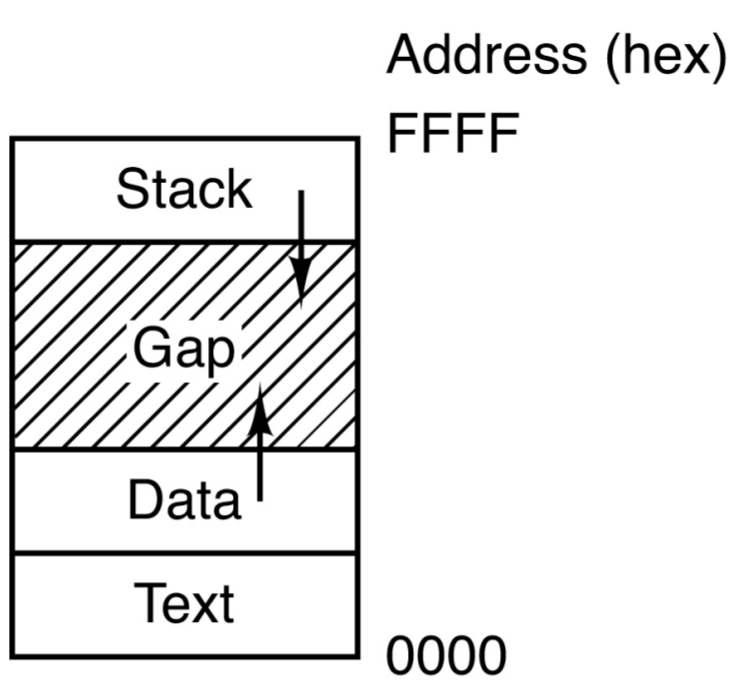
\includegraphics[width=0.15\textwidth]{AddressSpaceLayout}\end{figure}

\paragraph{OS Concepts --- Threads}
\begin{itemize}
	\item \textbf{Thread}: represents execution state of process ($ \geq 1 $ thread per process)
	\begin{itemize}
		\item \emph{IP}: stores currently executed instruction (address in \code{text} section)
		\item \emph{SP}: stores address of stack top ($ > 1 $ threads $ \to $ multiple stacks!)
		\item \emph{PSW}: contains flags about execution history (e.g. last calculation was 0 $ \to $ used in following jump instruction)
		\item more general purpose registers, floating point registers,...
	\end{itemize}
\end{itemize}
\begin{figure}[h]\centering\label{Threads}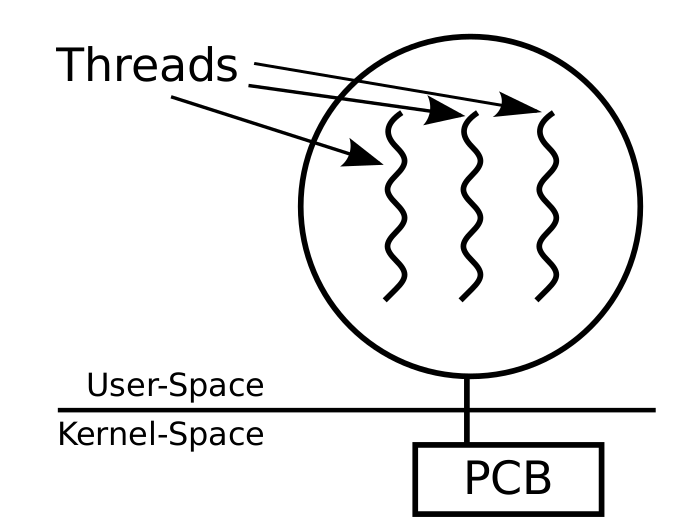
\includegraphics[width=0.2\textwidth]{Threads}\end{figure}

\paragraph{OS Concepts --- Policies vs. Mechanisms}
\begin{itemize}
	\item \textbf{Mechanism}: implementation of what is done (e.g. commands to write to HDD)
	\item \textbf{Policy}: rules which decide when what is done and how much (e.g. how often, how many resources are used,...)
	\item[$ \to $] \emph{mechanisms can be reused even when policy changes}
\end{itemize}

\paragraph{OS Concepts --- Scheduling}
\begin{itemize}
	\item \textbf{Motivation}: multiple processes/threads available $ \leadsto $ OS needs to switch between them (for multitasking)
	\item \textbf{Scheduler}: decides which job to run next (\emph{policy}) --- tries to
	\begin{itemize}
		\item provide fairness
		\item meet performance goals
		\item adhere to priorities 
	\end{itemize}
	\item \textbf{Dispatcher}: performs task-switching (\emph{mechanism})
\end{itemize}
\begin{figure}[h]\centering\label{Scheduling}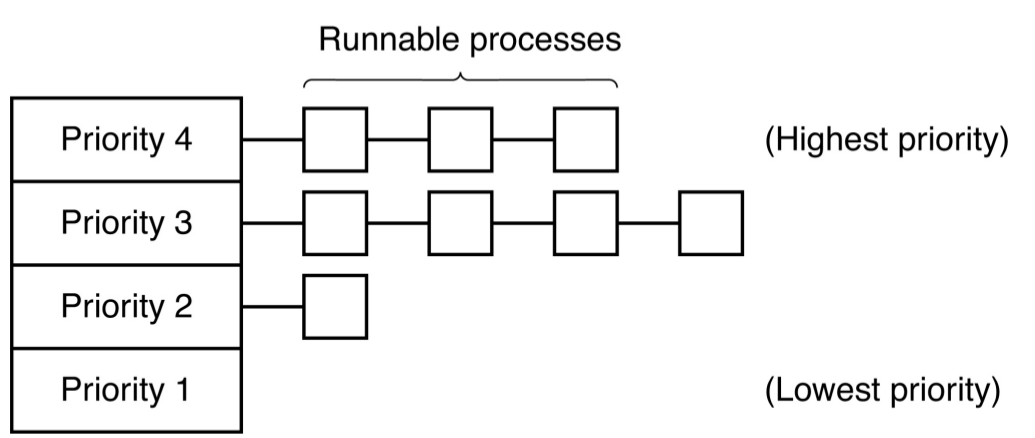
\includegraphics[width=0.33\textwidth]{Scheduling}\end{figure}

\paragraph{OS Concepts --- Files}
\begin{itemize}
	\item \textbf{Motivation}: OS hides peculiarities of file storage, programmer uses device-independent \emph{files}/\emph{directories}
	\item \textbf{Files}: associate \emph{file name} and \emph{offset} with bytes
	\item \textbf{Directories}: associate \emph{directory names} with directory names or file names
	\item \textbf{File System}: ordered block collection
	\begin{itemize}
		\item main task: translate (dir name + file name + offset) to block
		\item programmer uses file system operations to operate on files (\code{open}, \code{read}, \code{seek})
		\item processes can communicate directly through special \emph{named pipe} file (used with same operations as any other file)
	\end{itemize}
\end{itemize}

\paragraph{OS Concepts --- Directory Tree}
\begin{itemize}
	\item \textbf{Directories}: form \emph{directory tree}/\emph{file hierarchy}
		$ \to $ structure data
	\item \textbf{Root Directory}: topmost directory in tree
	\item \textbf{Path Name}: used to specify file
\end{itemize}

\paragraph{OS Concepts --- Mounting}
\begin{itemize}
	\item \textbf{Unix}: common to orchestrate multiple file systems in single file hierarchy
	\item file systems can be \emph{mounted} on directory
	\item \textbf{Win}: manage multiple directory hierarchies with drive letters (e.g. \code{C:\\Users})
\end{itemize}

\paragraph{OS Concepts --- Storage Management}
\begin{itemize}
	\item \textbf{OS}: provides uniform view of information storage to file systems
	\begin{itemize}
		\item \emph{Drivers}: hide specific hardware devices $ \to $ hides device peculiarities
		\item general interface abstracts physical properties to logical units $ \to $ block
	\end{itemize}
	\item \textbf{Performance}: OS increases I/O performance:
	\begin{itemize}
		\item \emph{Buffering}: Store data temporarily while transferred
		\item \emph{Caching}: Store data parts in faster storage
		\item \emph{Spooling}: Overlap one job's output with other job's input
	\end{itemize}
\end{itemize}

\begin{summary}
	\begin{itemize}
		\item \textbf{OS}: provides abstractions for and protection between applications
		\item \textbf{Kernel}: does not always run --- certain events invoke kernel
		\begin{itemize}
			\item \emph{syscall}: process asks kernel for service
			\item \emph{interrupt}: device sends signal that OS has to handle
			\item \emph{exception}: CPU encounters unusual situation
		\end{itemize}
		\item \textbf{Processes}: encapsulate resources needed to run program in OS
		\begin{itemize}
			\item \emph{threads}: represent different execution states of process
			\item \emph{address space}: all memory process can name
			\item \emph{resources}: allocated resources, e.g., open files
		\end{itemize}
		\item \textbf{Scheduler} decides which process to run next when multi-tasking
		\item \textbf{Virtual Memory} implements address spaces, provides protection between processes
		\item \textbf{File system} abstracts background store using I/O drivers, provides simple interface (files + directories)
	\end{itemize}
\end{summary}